

\documentclass[journal=jpcbfk,layout=traditional]{achemso}
%\documentclass[journal=jpcbfk,layout=twocolumn]{achemso}

\usepackage[utf8]{inputenc}

\usepackage{graphicx}
\usepackage{xcolor}

\usepackage{textgreek}
\usepackage{chemmacros}

\usepackage{siunitx}
\sisetup{list-units = single, range-units = single}
\DeclareSIUnit\rydberg{Ry}


%\newcommand{\todo}[1]{\textcolor{red}{\textbf{#1}}}

\newcommand{\Barbara}[1]{\textcolor{teal}{\textbf{#1}}}
\newcommand{\Carsten}[1]{\textcolor{blue}{\textbf{#1}}}
\newcommand{\Marco}[1]{\textcolor{purple}{\textbf{#1}}}
\newcommand{\Vahideh}[1]{\textcolor{brown}{\textbf{#1}}}


\title{chemHMC}
\author{Vahideh Alizadeh}
\affiliation{Mulliken Center for Theoretical Chemistry, University of Bonn, Beringstra\ss e 4+6, D-53115 Bonn, Germany}
\author{Marco Garofalo}
\affiliation{HISKP (Theory), Rheinische Friedrich-Wilhelms-Universität Bonn, Nussallee 14-16, 53115, Bonn, Germany}
\author{Carsten Urbach}
\email{urbach@hiskp.uni-bonn.de}
\affiliation{HISKP (Theory), Rheinische Friedrich-Wilhelms-Universität Bonn, Nussallee 14-16, 53115, Bonn, Germany}
\author{Barbara Kirchner}
\email{kirchner@thch.uni-bonn.de}
\affiliation{Mulliken Center for Theoretical Chemistry, University of Bonn, Beringstra\ss e 4+6, D-53115 Bonn, Germany}


\begin{document}


\begin{abstract}



   
  % bottlenecks??!!\\
 %Which kind of disadvantages exists in individual MD and MC methods that a combination of them (HMC) could solve? is there a different HMC? could we define various HMCs based on other MCs and MDs themselves and combinations ways? shadow-HMC\cite{izaguirre2004shadow}
\end{abstract}

%%%%%%%%%%%%%%%%%%%%%%%%%%%%%%%%%%%%%%%%
\section{Introduction}
%%%%%%%%%%%%%%%%%%%%%%%%%%%%%%%%%%%%%%%%%
Molecular simulations could be concisely described as computational statistical mechanics, i.e., numerical methods combined with computer power to address physico-chemical problems arising in condensed matter systems.\cite{ciccotti2022molecular} 
%Statistical mechanics is that branch of physics which studies macroscopic systems from a microscopic or molecular point of view. from mMcQuarrie-statistical mechanics


%(why we need HMC, highlight HMC advantage points)

%%%%%%%%%%%%%%%%%%%%%%%%%%%%%%%%%%%%%%%%%
\section{Theory}
%%%%%%%%%%%%%%%%%%%%%%%%%%%%%%%%%%%%%%%%%




HMC \cite{duane1987hybrid}

%%%%%%%%%%%%%%%%%%%%%%%%%%%%%%%%%%%%%%%%%
%\section{Computational details}
%%%%%%%%%%%%%%%%%%%%%%%%%%%%%%%%%%%%%%%%%

\newpage
%%%%%%%%%%%%%%%%%%%%%%%%%%%%%%%%%%%%%%%%%
\section{Workflow}
%%%%%%%%%%%%%%%%%%%%%%%%%%%%%%%%%%%%%%%%%

\begin{figure}
    \centering
   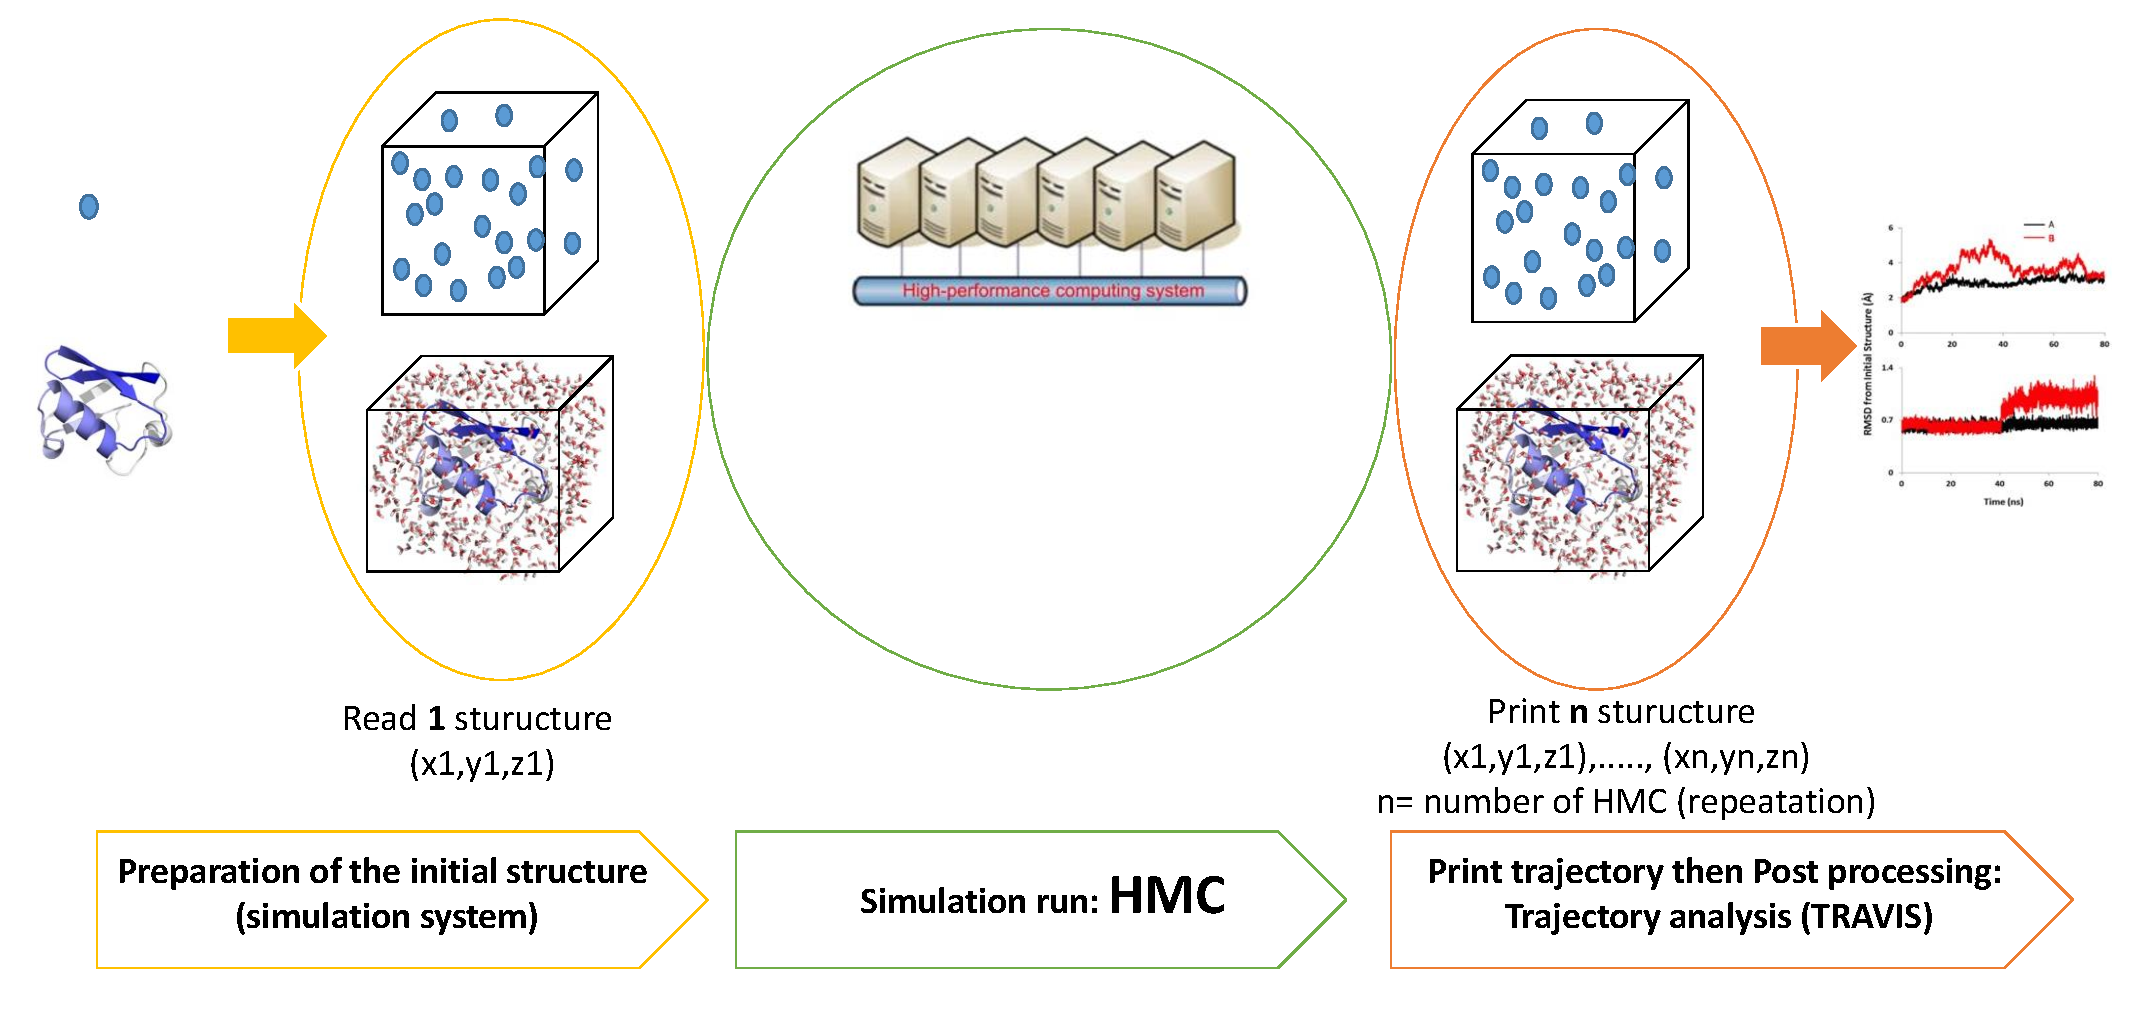
\includegraphics[width=0.9\columnwidth]{pics/schem1.pdf}
    \caption{General scheme of our goal within HMC project and code.}
    \label{fig:my_label}
\end{figure}

\subsection{The Algorithm}

\begin{enumerate}
    \item Input: arbitrary $q_i$ (positions), $U={U_i}$ (potential)
    \item for t= 1, 2,... do 
    \item generate $p_i$ (momenta) standard normal distributed
    \item integrates equation of the motion $f=m.a=$ for the trajectory of length t and find proposal $U'=U(t)$ and momenta P' using an integration scheme (the measures in phase space are reversible, invariant)
    \item accept U' with probability\\
    $P_{acc}=min{1, exp}$
\end{enumerate}
\subsection{Technical details}


\large\textbf{Code Layout}
\begin{itemize}
    \item main: main.cpp
    \item modules
    \item
    
\end{itemize}


\subsection{Case study: Melting via Lenard-Jones potential}




first case study: melting and crystalization of the LJ particles.
-- define these process 


-- why melting, crystallization, and LJ particles are interesting as the first case study?


-- what is the disadvantage of current workflows for studying them or in other words how HMC could be helpful to study this process?
(why we need HMC, highlight HMC advantage points)


--




%%%%%%%%%%%%%%%%%%%%%%%%%%%%%%%%%%%%%%%%%
%\section{Results}
%%%%%%%%%%%%%%%%%%%%%%%%%%%%%%%%%%%%%%%%%


%%%%%%%%%%%%%%%%%%%%%%%%%%%%%%%%%%%%%%%%%
\newpage
\section{Conclusions}
%%%%%%%%%%%%%%%%%%%%%%%%%%%%%%%%%%%%%%%%%


\begin{acknowledgement}
 
\end{acknowledgement}



\bibliography{ref}

\end{document}



